\subsection*{Effects of Display Size and Navigation Type on a Classification Task}
    \subparagraph{by : C.Liu, O.Chapuis, M.Beaudouin-Lafon, E.Lecolinet, W.Mackay}
    \cite{liu2017CoReach}
    \paragraph{ \textit{Quick Summary :} 
                \newline
                \indent \indent \textnormal{This research papers offers a set of Gestures that would allow users of LHRD to interact more
                easily with the contents they wanna manipulate. As the general multi-touch displays are using pretty common ones, these doesn't 
                scale well with a wall-sized display.}
                \newline
                \indent \indent \textnormal{In this paper, the main worked points are about co-located collaborative navigations, which involves
                more complex dynamics when you're aware of problems like "gorilla-arm" or simply the loss of precision for precise manipulation gestures. 
                Also the \textit{CoReach} set of gestures had to be thought taking care of multiples human factors, such as collaborative strtategies, 
                or even physical constraints.}
                \newline
                \indent \indent \textnormal{Especially, this research focuses on Collaborative interactions, as most (if not every) of the previous works
                did focus on addressing precision and fatigue problems for single-users. To recap, \textit{CoReach} focuses on Large Scale Interaction \& 
                MultiUser Cooperative Actions.} }
    
    \paragraph{ \textit{Motivations :} 
                \newline
                \indent \indent \textnormal{With the rise of dat-driven decision making, scenarios where people face communication barriers due to domain-specific 
                terms are becomming common place. And as a solution to this problem comes the large interactive spaces, and especially as we're talking about datas 
                visualization and manipulation, LHRDs !} }

    \paragraph{\textit{Gestures:} \newline}
    \indent \indent Obviously, what would be a set of gestures without any gestures ? So here is a scheme showing and explaning the three different
    implemented gestures for the \textit{CoReach} prototype :
    
                
    \begin{figure}[h]
        \centering
        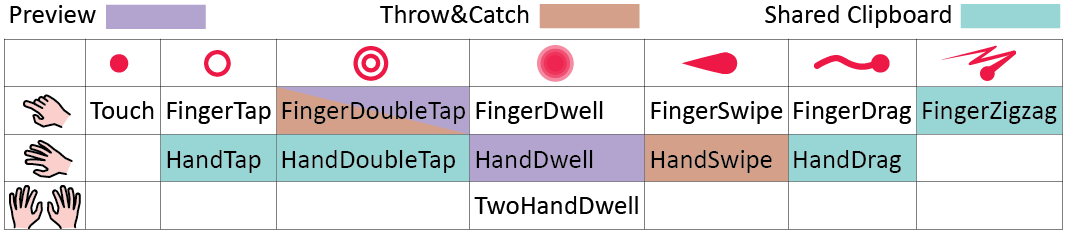
\includegraphics[width=0.5\textwidth]{images/RecognizedGestures.png}
        \caption{Figure 1. image taken from the source article (Fig2)}
        \label{fig:myimage}
    \end{figure}
    
    \indent \indent So these three recognized gestures were implemented in the prototype, and they're meant to facilitate data-centric
    collaborative tasks on large interactive surfaces. Plus these are especially the pattern gestures that can be applied \& used by a couple of users in a 
    tasks. Below are detailled these three different gestures and their uses.

    \begin{itemize}
        \item \textit{Throw and Catch :} \newline 
        \item \textit{Preview :} \newline 
        \item \textit{Shared Clipboard} \newline 
    \end{itemize}

    \paragraph{ \textit{Study 1 :}
                \newline}
    
    \paragraph{ \textit{Study 2 :}
                \newline 
                \indent \indent \textnormal{} }
            
    \paragraph{ \textit{Discussion :}
                \newline
                \indent \indent \textnormal{} }
    
    \paragraph{ \textit{Conclusion :}
                \newline
                \indent \indent \textnormal{} }
    